\title{\vspace{160px} \textbf{\huge{Telecommunication Theory}} \\\vspace{17.5px} \LARGE{Lab report 3}  \vspace{10px}}
\author{Alessandro Trigolo}
\date{December 4, 2023}

\begin{document}
\maketitle \newpage

\section*{Objective}
This laboratory work's goal is to prepare the code that will be used in both lab 4 and lab 5. In this lab work the three modulation techniques - \textsl{BASK}, \textsl{BFSK} and \textsl{BPSK} - will be prepared for the following labs: the initial binary data sequence will be modulated and then the \textsl{Gaussian White Noise} will be added to the signal. However, in the laboratory work, the noise won't be added using the \texttt{awgn} function but will be generated with a script.

\section*{Source code and plots}
\lstset{style = MatLab}
The MATLAB source code produced to accomplish this lab work is presented in this section. Alongside the lines of code, there will be some explanatory comments to make the source code more readable. It is important to notice that the \textsl{Task 4} and the \textsl{Task 5} have been incorporated inside the \textsl{Task 2} and the \textsl{Task 3} to increase the clarity of the report.

\subsection*{Task 1}
The first task of the laboratory work asked to set up a random binary data sequence and initialize some parameters that will be needed in the following task such as the symbol duration $T$, the carrier frequency $f_0$, the number of symbols $N$ and the \textsl{SNR} value. The first task is the same for all of the three types of modulation. After generating the random number of \textit{N} binary symbols, the plotting has been achieved by the MATLAB \texttt{step} function. 

\begin{lstlisting}
% Parameters for the signal generation 
T = 1; % symbol duration [seconds]
F0 = 10; % carrier frequency [Hz]
N = 15; % number of symbols
binary_sequence = randi(2, 1, N) - 1; % random sequence of 1 and 0
SNR = 15; % Db

% Create figure
f = figure(1);
f.Position = [450, 100, 700, 600];
f.Name = 'BASK';

% plot the random binary sequence
subplot(311), stairs(0 : T : N * T, [binary_sequence binary_sequence(end)]), grid on; % plot
xlabel('Time [s]'), ylabel('Binary data'); % labels
ylim([-0.1 1.1]); % limits
\end{lstlisting}

\noindent After running this script the data will be displayed in the following way.

\begin{figure}[!h]
    \centering
    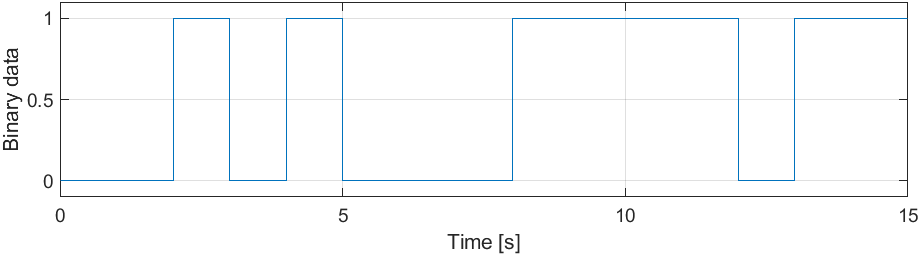
\includegraphics[width = .7\textwidth]{lab-3/imgs/task1.png}
\end{figure}
\vspace*{-15px}


\subsection*{Task 2}
Task number two asked to generate the specific modulated signal and display it in the second plot. The three plots will be properly discussed in the following paragraphs.

\subsubsection*{BASK}
The first modulation technique that we are going to plot is the \textsl{Binary Amplitude Shift Keying}. As we know, in the BASK modulation, the difference between the transmission of a 0 and a 1 is the carrier sine amplitude. Precisely, when the symbol is zero the amplitude is none, otherwise, the amplitude is one.

The code snippet below contains the script used to generate the BASK signal. Firstly it is necessary to create the carrier signal $s_0$ and then compose it with the initial random binary sequence using the \textsl{Kroneker} multiplication to get the actual BASK signal.

\begin{lstlisting}
% create carrier signal
delta_t =  T / 200; % step duration
t = 0 : delta_t : T - delta_t; % time intervals
s0 = sin (2 * pi * F0 * t); % carrier signal


% Generate BASK signal with no noise
BASK_signal = kron(binary_sequence, s0); % Kroneker multiplication
BASK_intervals = 0 : delta_t : N * T - delta_t; % time intervals for BASK 

subplot(312), plot(BASK_intervals, BASK_signal), grid on; % plot
xlabel('Time [s]'), ylabel('BASK signal'); % labels
ylim([-1.1 1.1]); % limits
\end{lstlisting}

\noindent After plotting the newly modulated signal the result is the one shown in the image below. Noticeably, when the sequence value is 0 the amplitude is none while when the symbol is one the amplitude becomes 1.

\begin{figure}[!h]
    \centering
    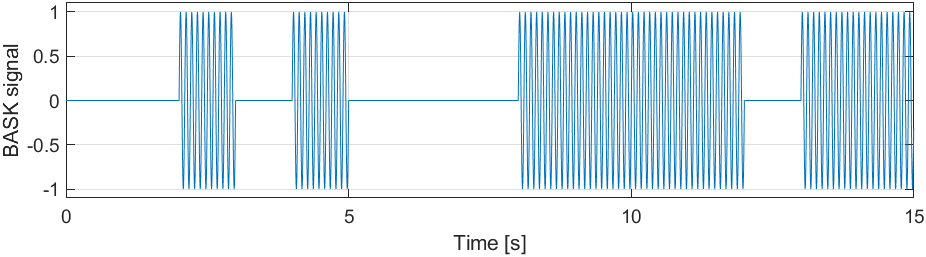
\includegraphics[width = .7\textwidth]{lab-3/imgs/task2_BASK.png}
\end{figure}
\vspace*{-15px}

\subsubsection*{BFSK}
The second modulation technique that we are going to plot is the \textsl{Binary Frequency Shift Keying}. In The BASK modulation, the difference between the transmission of a 0 and a 1 is the frequency of the carrier signal. In this case, the symbol zero leads to a carrier signal whose frequency is higher than the carrier signal associated with the symbol 1. 

In this case, to generate the BFSK signal the code is a little longer because the carrier signals are two instead of one. First of all, it is important to define the two carrier frequencies, $f_1$ and $f_2$ which differ $\pm\Delta f$ from the initial frequency $f_0$. At this point, we can calculate the two carrier signals, $s_1$ and $s_2$ that will be respectively associated with the symbol 1 and 0. The BFSK signal is the sum of the two BASK signals that are complementary to one another.

\begin{lstlisting}
% calculate f1 and f2 frequencies
k = 12;
delta_f = k /(2 * T); 
f1 = f0 - delta_f/2; % first frequency
f2 = f0 + delta_f/2; % second frequency

% create carrier signal
delta_t =  T / 200; % step duration
t = 0 : delta_t : T - delta_t; % time intervals
s1 = sin (2 * pi * f1 * t); % first carrier signal
s2 = sin (2 * pi * f2 * t); % second carrier signal


% Generate BFSK signal with no noise
BASK_signal_1 = kron(binary_sequence, s1); % Kroneker multiplication
BASK_signal_2 = kron(~binary_sequence, s2); % Kroneker multiplication
BFSK_signal = BASK_signal_1 + BASK_signal_2; % add together the two BASK signals
BFSK_intervals = 0 : delta_t : N * T - delta_t; % time intervals for BFSK
\end{lstlisting}

\noindent The result of the BFSK signal plot is shown in the figure below. Noticeably, when a 0 occurs the frequency is higher and it's lower when a 1 is transmitted.

\begin{figure}[!h]
    \centering
    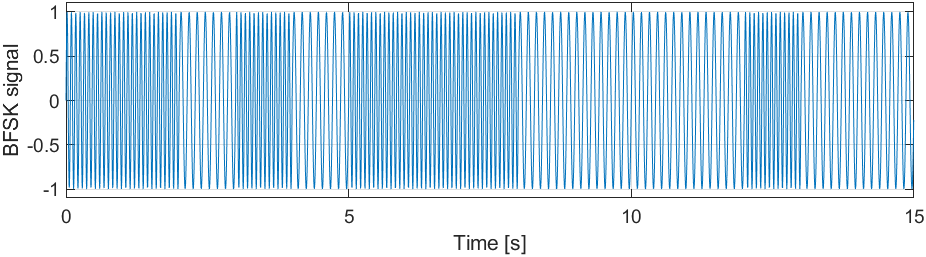
\includegraphics[width = .7\textwidth]{lab-3/imgs/task2_BFSK.png}
\end{figure}
\vspace*{-15px}

\subsubsection*{BPSK}
The last modulation type is the \textsl{Binary Phase Shift Keying}. In the BPSK the difference between the symbol 1 and 0 is the phase of the wave signal. The phase shift is always $\pi$ which means that the carrier for the symbol 1 is the opposite signal of the carrier of the symbol 0. This makes this modulation the most effective among the three.

The procedure for generating the carrier signal is the same as for the BASK modulation. To create the BPSK signal it is necessary to convert the random binary data sequence into an NRZ (\textsl{Non-Retur-to-Zero}) signal. In such a way, when the Kroneker multiplication generates the signal, the carrier signal will be the opposite for one symbol. 

\begin{lstlisting}
% create carrier signal
delta_t =  T / 200; % step duration
t = 0 : delta_t : T - delta_t; % time intervals
s0 = sin (2 * pi * F0 * t); % carrier signal


% Generate BPSK signal with no noise
NRZ_binary_sequence = -2 * binary_sequence + 1; % convert initial data into NRZ signal
BPSK_signal = kron(NRZ_binary_sequence, s0); % Kroneker multiplication
BPSK_intervals = 0 : delta_t : N * T - delta_t; % time intervals for BPSK 

subplot(312), plot(BPSK_intervals, BPSK_signal), grid on; % plot
xlabel('Time [s]'), ylabel('BPSK signal'); % labels
ylim([-1.1 1.1]); % limits
\end{lstlisting}

\noindent After plotting the BPSK modulation (shown below) we can notice that when there is a switch between two symbols the phase of the carrier changes by $\pi$.

\begin{figure}[!h]
    \centering
    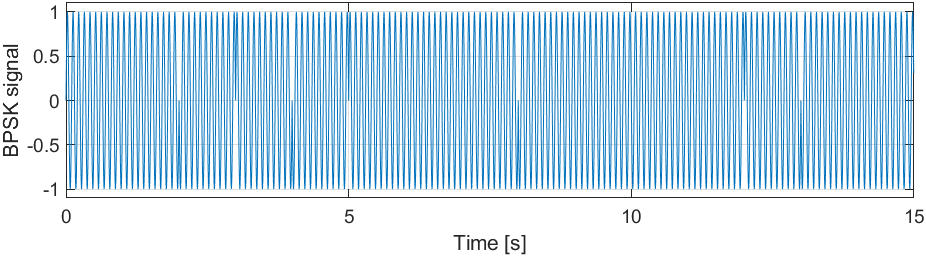
\includegraphics[width = .7\textwidth]{lab-3/imgs/task2_BPSK.png}
\end{figure}
\vspace*{-15px}

\subsection*{Task 3}
The third task requested to add the \textsl{Additive Gaussian White Noise} to the modulated signal. In this case, the noise has not been added with the \texttt{agwn} function but through the following script, which is the same for the three modulation techniques. By reversing the \textsl{SNR} formula it is possible to get the value of $E_bN_0$ and after calculating the carrier energy $E_b$ the value of $N_0$, which is the noise power spectral density, is easy to reach. With this value, it is then possible to calculate the noise.

\begin{lstlisting}
% Generate AGWN
EbN0 = 10^(SNR / 10); % inversed SNR formula
Eb = sum(s0.^2); % energy of carrier signal
N0 = Eb / EbN0; % noise power spectral density
sigma = sqrt(N0 / 2); % sigma^2 = N0/2
noise = sigma * randn(1, N * 200); % get gaussian noise using randn()
\end{lstlisting}

\noindent After generating the noise, the only thing to do before plotting the disturbed modulated signal is to add the noise to the signal. In the code snipped below, there is the script used for the BPSK signal but for the two modulation types, the script is the same.

\begin{lstlisting}
% Add noise to the BPSK signal
BPSK_with_noise = BPSK_signal + noise;
subplot(313), plot(BPSK_intervals, BPSK_with_noise), grid on; % plot
xlabel('Time [s]'), ylabel('BPSK signal with noise'); % labels
ylim([-4, 4]); % limits
\end{lstlisting}

\noindent Now we can plot the three different disturbed modulated signals. The three figures below respectively show the plot of BASK, BFSK and BPSK.
\begin{figure}[!h]
    \centering
    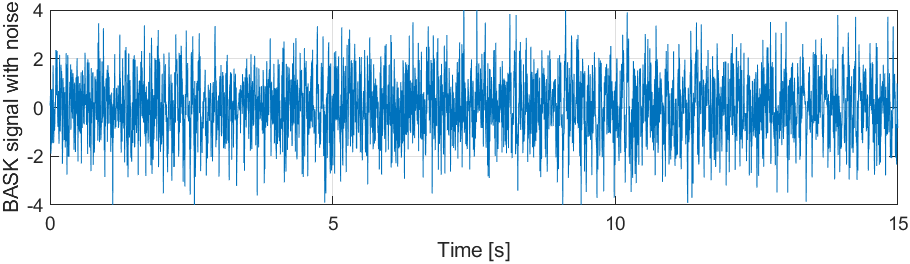
\includegraphics[width = .7\textwidth]{lab-3/imgs/task3_BASK.png}
    \caption*{The BASK disturbed signal.}
\end{figure}
\vspace*{-15px}
\begin{figure}[!h]
    \centering
    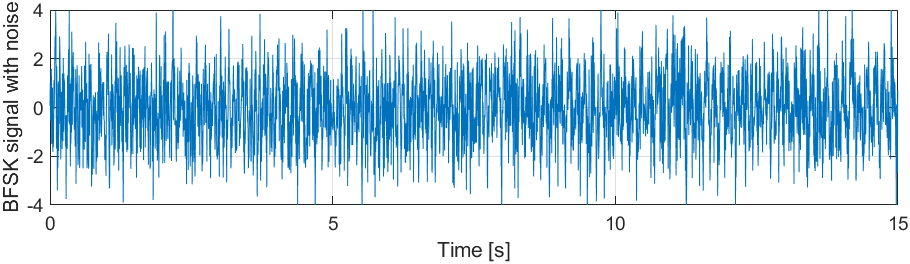
\includegraphics[width = .7\textwidth]{lab-3/imgs/task3_BFSK.png}
    \caption*{The BFSK disturbed signal.}
\end{figure}
\vspace*{-15px}
\begin{figure}[!h]
    \centering
    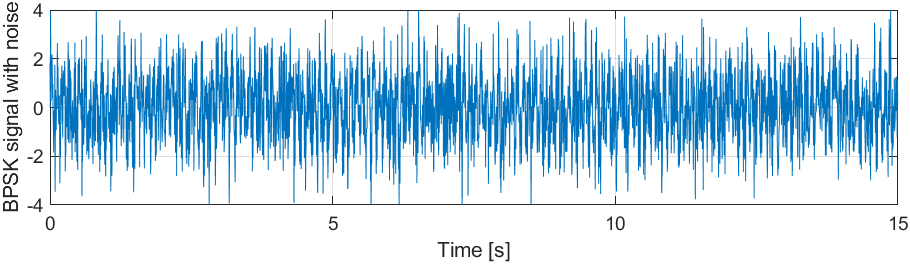
\includegraphics[width = .7\textwidth]{lab-3/imgs/task3_BPSK.png}
    \caption*{The BPSK disturbed signal.}
\end{figure}
\vspace*{-15px}

\section*{Conclusions}
By only observing the disturbed modulated signal, due to the high interference of the Gaussian Noise, it is rather difficult to even distinguish which modulation type was used. Reasonably, as the SNR increases the noise impact on the modulated signal will decrease making the signal more visually recognizable. Nonetheless, even though by only using the naked eye it is hardly possible to distinguish the signal, in the next labs there will be some techniques that will properly detect the initial binary sequence by analyzing the disturbed signal. 




\end{document}